\chapter{Теоретичні відомості}

\section{Нахождение абсолютного расстояния методом бинокулярного параллакса}
\subsection{О камерах}

В нашем случае в качестве ''глаза'' используется камера, поэтому для последующих выкладок нам нужно иметь представление о том, как она устроена и как работает.

Сегодня существует множество разных типов камер, и хоть каждая из них может иметь свои особенности конструкции, базовый принцип работы у них у всех одинаковый.
Основа камеры -- её светочувствительная матрица. В ней свет преобразуются в поток цифровых данных, непосредственно формируя изображение. После неё обычно находится объектив. Он отвечает за проекцию изображения на матрицу, позволяя регулировать фокусное расстояне, значение диафрагмы и другие параметры. 
	
\includegraphics[scale = 0.75]{placeholder}
		
	Рассмотрим принцип работы камеры на примере камеры-обскуры. 
	
		
\includegraphics[scale = 0.75]{placeholder}

В силу оптических особенностей, конечное изображение в такой камере будет перевернутым. Поэтому для ещё большего упрощения мысленно перенесём матрицу камеры направо, на расстояние $f$. Такое действие никак не повлияет на итоговый результат, но сильно упростит дальнейшие выкладки.

Покажем теперь, как с помощью двух таких камер можно найти абсолютное расстояние до объекта. Пусть пока камеры будут расположены параллельно и сонаправленны друг другу (что делать в случае когда камеры рассположены иначе будет указано дальше).
Итак, у нас есть такая конструкция:
	
		
\includegraphics[scale = 0.75]{placeholder}
	
	Где $f$ -- фокусное расстояние камеры, $\Delta$ -- расстояние между камерами, $z$ -- искомая глубина изображения, $x_1, x_2$ -- координата объекта на левом и на правом снимке, $R, L$ -- оптические центры правой и левой камеры, $S$ -- объект.\\
	
	Тогда из подобия треугольников следует:\\
	$$\begin{cases} \frac{f}{x_1} = \frac{z}{\Delta + x} \\ \frac{f}{x_2} = \frac{z}{x} \end{cases}$$
	
	Выразив $\Delta$ из первого уравнения, и $x$ из второго получим:\\
	$$\begin{cases} \Delta = \frac{z x_1}{f} - x \\ x = \frac{zx_2}{f} \end{cases}$$
	
	Подставим $x$ в первое уравнение и выразим из получившегося $z$\\
	$$ z = \frac{\Delta f}{(x_1 - x_2)}$$
	
	Так как $\Delta$ и $f$ не зависят от расположения объекта, а являются характеристиками самой камеры, то расстояние до объекта зависит только от разницы $x_1 - x_2$, то есть только от смещения объекта между двумя снимками. Следовательно для нахождения карты глубин нам нужно найти "сдвиг" для каждого пикселя.\\
	
\subsection{!!Ректификация!!}	
	Но для того чтобы вычислить $x_1 - x_2$ нужно сначала найти эту пару соответствующих пикселей, а это сложная задача. Для каждого пискселя левого изображения, нам нужно найти соответствующий среди пикселей правого изображения. Нужно ли нам перебирать все пиксели правого изображения, или всё таки можно ограничиться каким-то подмножеством пикселей?\\
	
	Пусть у нас есть изображение какого-то объекта на фоне стены.
	$$Рисунок 6$$
	
	Всё что мы можем сказать о его рассположении относительно камеры, это что он находится где-то на луче $L$.
	
	
\includegraphics[scale = 0.75]{placeholder}
	
	Добавим теперь вторую камеру, на каком-то расстоянии $\Delta$ от первой камеры. Если мы теперь проведем лучи из оптического центра правой камеры так, чтобы они пересекали луч $L$ - мы получим, так называемые, "эпиполярные линии". И теперь мы можем сократить множество для поиска соответствующих пар со всего изображения до эпиполярных линий на нём. Это существенно облегчает нам задачу.
	
	
\section{Стерео-зрение при полных данных}
Для простоты в этой работе рассматриваются только одномерные алгоритмы поиска карт сдвигов. Это означает, что каждую строку изображения мы обрабатываем независимо от других. Такой подход требует предварительной ректификации изображения, однако является более быстрым и дает неплохие результаты (рис. \ref{results}).
\begin{figure}
	\centering
	
\includegraphics[scale = 0.75]{placeholder}
	\caption{построчная карта сдвигов}
	\label{results}
\end{figure}
	
	Однако не любая пара пикселей может находиться в соответсвии! Пикселю левого изображения с номером $i$ могут соответсвовать только $i-k$ -е  пиксели правого изображения ($k = (0,i-1)$). Вы можете убедиться в этом держа перед собой карандаш и поочередно закрывая то правый, то левый глаз. В правом глазу карандаш будет находиться левее чем в левом.
	$$Рисунок 9$$
	
	Но всё же, как нам искать соответствующие пиксели? Какими характеристиками обладают соответствующие пиксели? Логично было бы предположить, что у них одинаковый цвет. Но этого не достаточно. Тогда можно ещё посмотреть какие свойства есть у соседних соответствующих пикселей. Допустим для пикселя $x_{i}$ уже найден соответствующий ему пиксель, то есть нам уже известне сдвиг для $(i)$-го пикселя. Можем ли мы что-то сказать о сдвиге для $(i+1)$-го пикселя? Так как всё же большинство объектов в реальной жизни - гладкие, то велика вероятность, что сдвиг для $(i+1)$-го пикселя не будет сильно отличаться от сдвига $(i)$-го пикселя. Иными словами в последовательности сдвигов должно быть мало скачков.\\
	
	Итак, у нас есть два признака похожести пикселей: схожесть цветов и схожесть соседних сдвигов. Введём качественные оценки этих двух характеристик. Схожесть цветов определим как расстояние между ними, в их цветовом пространстве (!опасный момент!). Схожесть же соседних сдвигов определим просто как модуль разности значений этих сдвигов.\\
	
	Поставим задачу более формально. Пусть множество 
	$\mathcal{L} = \{x_i \; | \; i = \overline{1,\, n}\}$ --- левое изображение-строка, $n$ - ширина изображения, $x_i$ - цвет пикселя (если у нас черно-белые 8-битные изображения, то $x_i \in [ \, 0, \; 255 \,]$, если же цветные, то $x_i \in {[ \, 0, \; 255 \,]}^3$). Введём функцию $\mathcal{L}(i)$ --- цвет $i$-го пискеля на левом изображении. Аналогично, $\mathcal{R}$ --- правое изображение-строка, а $\mathcal{R}(i)$ --- цвет $i$-го пискеля на правом изображение.
	
	Для каждого пикселя $i$ левого изображения нам нужно найти соответствующий ему пиксель на правом изображении, то есть найти такой сдвиг $d_i$, что:
	\begin{enumerate}
	
	\item Мимимизирует \textbf{Унарный штраф} $H(i, d) = | \, \mathcal{L}(i)- \mathcal{R}(i - d) \, |$\\
	(!норма, а не модуль!)
	
	\item Мимимизирует \textbf{Бинарный штраф} $g(d, d') = \alpha \, | \; d - d' \; |$ \\
	(где  --- $\alpha$ коэффициент сглаживания, и подбирается экспериментально)
	
	\end{enumerate}
	
			
	
	Можем построить штрафную функцию 
	$\omega (\overline{d}) = \sum\limits_{i=1}^n H(i, d_i) + \sum\limits_{i=1}^{n-1} g(d_i, d_{i+1})$
	
	Тогда, такая последовательность $\overline{d}$ которая минимизирует штрафную функцию $\omega (\overline{d})$ и будет нашим решением. Таким образом имеем задачу оптимизации.
	
	Для нахождения эффективного решения, и большего понимания задачи,  представим её в несколько ином виде, а именно в виде ориентированного графа. 
	
	Множество вершин $V = \{ \; \sigma(i, d) \, | \, i = \overline{(1,\, n)}, \, d = \overline{(0, \, maxD )} \; \} \bigcup \{\,S, E\,\}$.\\
	Вес вершины $\sigma(i, d) = H(i, d) \;, \; i = \overline{(1,\, n)}, \, d = \overline{(0, \, maxD )}$\\
	Веса ребёр: 
	\begin{enumerate}
	\item Из $S$ в $\sigma(1, d)$ вес ребра = $0$, $d = \overline{(0,\, maxD)}$
	\item Из $\sigma(n, d)$ в $E$ вес ребра = $0$, $d = \overline{(0,\, maxD)}$
	\item Из $\sigma(i, d)$ в $\sigma(i+1, d')$ вес ребра = $q(d, d')$, $d, d' = \overline{(0,\, maxD)}$
	\end{enumerate}	
	
	Получается такой граф:
	$$Рисунок 10$$

 	
 	Тогда, длина пути из вершины $S$ в вершину $E$ через вершины $\sigma(i, d)$ где $i = \overline{(1,\, n)}$, а $d \in \overline{d}$ будет равна:
 	$$\sum\limits_{i=1}^n H(i, d_i) + \sum\limits_{i=1}^{n-1} g(d_i, d_{i+1})$$
 	
	Что в точности повторяет нашу штрафню функцию, причём последовательность $\overline{d}$ минимизирующая эту штрафню функцию, будет отвечать последовательности вершин, которые составляют самый короткий путь из вершины $S$ в вершину $E$.
	
	Таким образом наша задача сводится к поиску кратчайшего пути на графе.\\
	
	Решать эту задачу традиционными алгоритмами типа Белмана-Форда или Дейкстры - не самая лучшая идея. Алгоритм Белма-Форда имеет сложность $|V| * |E|$, причём $|E|$ у нас равна $D^2 n$, где $D$ - максимальный диспаритет, $n$ - ширина изображения.
	
	Куда эффективнее решать эту задачу при помощи ДИНАМИЧЕСКОГО ПРОГРАМИРОВАНИЯ. \\
	
	Обозначим длину кратчайшего пути из вершины S в вершину $\sigma(i, d)$ как $f_i(d)$. 
	Тогда для любого $d \in D$:\\
	
		$f_1(d) = H(1, d)$
		
		$f_2(d) = \min(H(1,d') + g(d', d)) = \min(f_1(d') + g(d', d)) + H(2,d)$
		
	 	...
	 	
	 	$f_n(d) = \min(f_{n-1}(d') + g(d', d)) + H(n,d)$\\

	А саму последовательность $\overline{d}$ находим так:\\
	
		$d_m = arg\min_{d'} (f_m(d'))$
		
		$d_i = arg\min_{d'} (f_i(d') + H(i,d'))$	
\section{Стерео-зрение при неполных данных}

%%===========================================================================%%
\section{Стерео-зрение при медленно поступающих данных}
%%===========================================================================%%
\newpage
%%-------------------------------------------------%%
\subsection{Данные приходят по порядку}
%%-------------------------------------------------%%
Пусть сначала все пиксели нам неизвестны (рис. \ref{1.4_im_nodata}), поэтому мы не можем вычислить вес ни одной из вершин графа $G$ ( \ref{Def_G}).
%2.1nodata
\begin{figure}[h!]
	\centering
	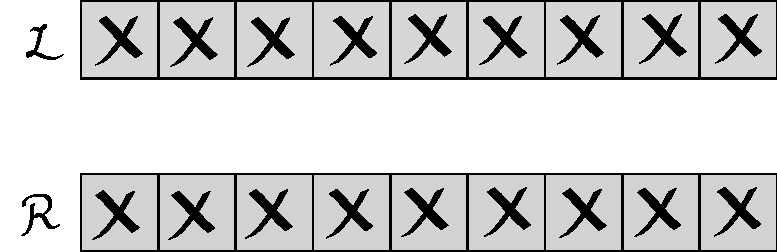
\includegraphics[scale = 0.7]{allclosed2.pdf}
	\caption{Нет данных}
	\label{1.4_im_nodata}
\end{figure}

\label {2.1-style} Если мы не можем вычислить вес вершины --- будем называть эту вершину ''\textit{закрытой}'' и обозначать ее черным кружочком. В противном случае назовем вершину ''\textit{открытой}'' и обозначим белым кружком. Для простоты рисунков положим $ D_{max} = 2 $ и не будем обозначать ребер. Тогда, в ситуации когда все данные нам неизвестны, граф $ G $ будет иметь следующий вид (рис. \ref{1.4Gnodata}). 
%Gnodata
\begin{figure}[h!]
	\centering
	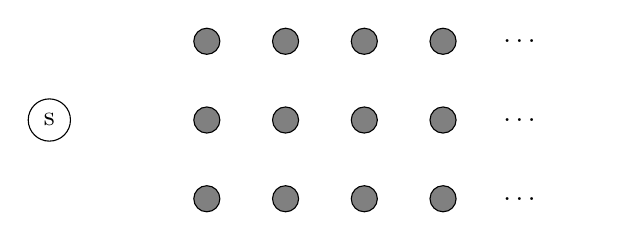
\begin{tikzpicture}[scale=1]
	\tikzstyle{vertex_closed_1} = [circle, draw=black, fill=gray, opacity=0.3]
	\tikzstyle{vertex_closed_2} = [circle, draw=black, fill=gray]
	\tikzstyle{vertex_opened} = [circle, draw=black]

%------------------------------------------------------------
	\node[vertex_opened] (s) at (-1,1) {s};

	\node[vertex_closed_2] (v00) at (1,0) {};
	\node[vertex_closed_2] (v01) at (1,1) {};
	\node[vertex_closed_2] (v02) at (1,2) {};
		
%------------------------------------------------------------
	
	\node[vertex_closed_2] (v10) at (2,0) {};
	\node[vertex_closed_2] (v11) at (2,1) {};
	\node[vertex_closed_2] (v12) at (2,2) {};
		
%------------------------------------------------------------
	
	\node[vertex_closed_2] (v20) at (3,0) {};
	\node[vertex_closed_2] (v21) at (3,1) {};
	\node[vertex_closed_2] (v22) at (3,2) {};
		
%------------------------------------------------------------
	
	\node[vertex_closed_2] (v30) at (4,0) {};
	\node[vertex_closed_2] (v31) at (4,1) {};
	\node[vertex_closed_2] (v32) at (4,2) {};
		
%------------------------------------------------------------

	\node[vertex_closed_2, opacity =0] (v40) at (6,0) {};
	\node[vertex_closed_2, opacity =0] (v41) at (6,1) {};
	\node[vertex_closed_2, opacity =0] (v42) at (6,2) {};
	
	\path (v30) -- node[auto=false]{\ldots} (v40);
	\path (v31) -- node[auto=false]{\ldots} (v41);
	\path (v32) -- node[auto=false]{\ldots} (v42);
	
	\end{tikzpicture}
	\captionof{figure}{граф $G$ в отсутствии данных}
	\label{1.4Gnodata}
\end{figure}

Пусть теперь нам по порядку начинают приходить пары из пикселей правого и левого изображений с одинаковыми координатами. Когда нам известен только один первый пиксель каждого изображения (рис.\ref{1.4_im_onepixel}) то мы можем вычислить вес только одной вершины, и граф $G$ будет иметь вид как на рис.\ref{1.4_pl_Gonepixel}.
%1.4_im_onepixel
\begin{figure}[h!]
	\centering
	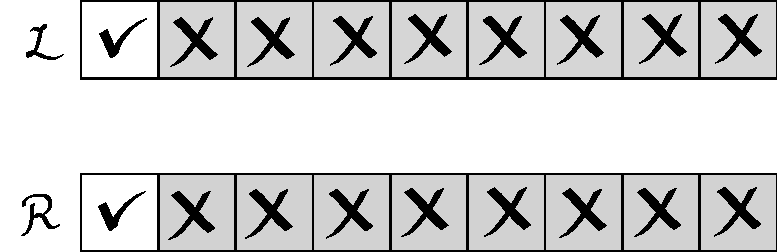
\includegraphics[scale = 0.7]{onestereoknown.pdf}
	\caption{Известны только первые пиксели}
	\label{1.4_im_onepixel}
\end{figure}
%1.4_pl_Gonepixel
\begin{figure}[h!]
	\centering
	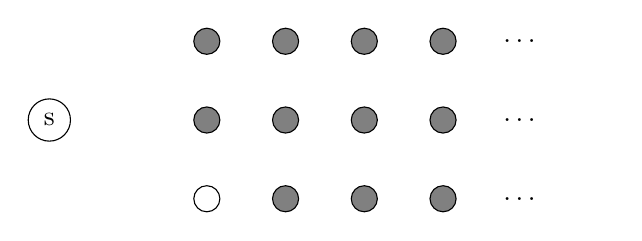
\begin{tikzpicture}[scale=1]

	\tikzstyle{vertex_closed_1} = [circle, draw=black, fill=gray, opacity=0.3]
	\tikzstyle{vertex_closed_2} = [circle, draw=black, fill=gray]
	\tikzstyle{vertex_opened} = [circle, draw=black]

%------------------------------------------------------------
	\node[vertex_opened] (s) at (-1,1) {s};

	\node[vertex_opened] (v00) at (1,0) {};
	\node[vertex_closed_2] (v01) at (1,1) {};
	\node[vertex_closed_2] (v02) at (1,2) {};
		
%------------------------------------------------------------
	
	\node[vertex_closed_2] (v10) at (2,0) {};
	\node[vertex_closed_2] (v11) at (2,1) {};
	\node[vertex_closed_2] (v12) at (2,2) {};
		
%------------------------------------------------------------
	
	\node[vertex_closed_2] (v20) at (3,0) {};
	\node[vertex_closed_2] (v21) at (3,1) {};
	\node[vertex_closed_2] (v22) at (3,2) {};
		
%------------------------------------------------------------
	
	\node[vertex_closed_2] (v30) at (4,0) {};
	\node[vertex_closed_2] (v31) at (4,1) {};
	\node[vertex_closed_2] (v32) at (4,2) {};
		
%------------------------------------------------------------

	\node[vertex_closed_2, opacity =0] (v40) at (6,0) {};
	\node[vertex_closed_2, opacity =0] (v41) at (6,1) {};
	\node[vertex_closed_2, opacity =0] (v42) at (6,2) {};
	
	\path (v30) -- node[auto=false]{\ldots} (v40);
	\path (v31) -- node[auto=false]{\ldots} (v41);
	\path (v32) -- node[auto=false]{\ldots} (v42);
	
	\end{tikzpicture}
	\captionof{figure}{Граф $G$ когда известны только первые пиксели}
	\label{1.4_pl_Gonepixel}
\end{figure}

Когда же нам будут известны уже первые два пикселя обоих изображений, мы сможем найти веса уже трёх вершин, и граф $G$ будет выглядеть как на рис.\ref{1.4_pl_twopixels}.
%G1.4_pl_twopixels
\begin{figure}[h!]
	\centering
	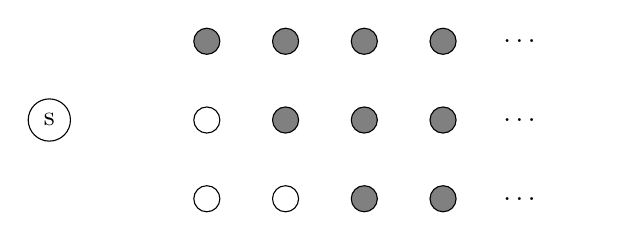
\begin{tikzpicture}[scale=1]
	\tikzstyle{vertex_closed_1} = [circle, draw=black, fill=gray, opacity=0.3]
	\tikzstyle{vertex_closed_2} = [circle, draw=black, fill=gray]
	\tikzstyle{vertex_opened} = [circle, draw=black]

%------------------------------------------------------------
	\node[vertex_opened] (s) at (-1,1) {s};

	\node[vertex_opened] (v00) at (1,0) {};
	\node[vertex_opened] (v01) at (1,1) {};
	\node[vertex_closed_2] (v02) at (1,2) {};
		
%------------------------------------------------------------
	
	\node[vertex_opened] (v10) at (2,0) {};
	\node[vertex_closed_2] (v11) at (2,1) {};
	\node[vertex_closed_2] (v12) at (2,2) {};
		
%------------------------------------------------------------
	
	\node[vertex_closed_2] (v20) at (3,0) {};
	\node[vertex_closed_2] (v21) at (3,1) {};
	\node[vertex_closed_2] (v22) at (3,2) {};
		
%------------------------------------------------------------
	
	\node[vertex_closed_2] (v30) at (4,0) {};
	\node[vertex_closed_2] (v31) at (4,1) {};
	\node[vertex_closed_2] (v32) at (4,2) {};
		
%------------------------------------------------------------

	\node[vertex_closed_2, opacity =0] (v40) at (6,0) {};
	\node[vertex_closed_2, opacity =0] (v41) at (6,1) {};
	\node[vertex_closed_2, opacity =0] (v42) at (6,2) {};
	
	\path (v30) -- node[auto=false]{\ldots} (v40);
	\path (v31) -- node[auto=false]{\ldots} (v41);
	\path (v32) -- node[auto=false]{\ldots} (v42);
	
	\end{tikzpicture}
	\captionof{figure}{Відомі перші два пікселі зображень}
	\label{1.4_pl_twopixels}
\end{figure}

По мере прихода следующих пикселей в графе $G$ будут открываться вершины на диагонали над уже открытыми вершинами. А как только нам станут известны $D_{max} + 1$ первых пикселей обоих изображений --- то все вершины в первом столбике станут открытыми (рис. \ref{1.4_pl_Dpixels}), и мы можем приступать к предвычислениям  
%1.4_pl_Dpixels
\begin{figure}[h!]
	\centering
	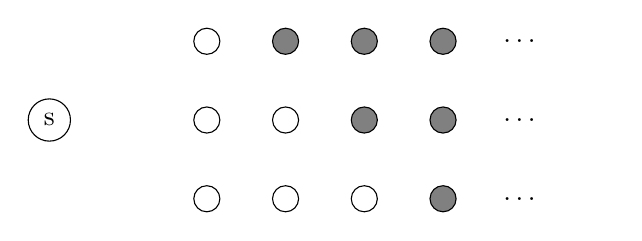
\begin{tikzpicture}[scale=1]

	\tikzstyle{vertex_closed_1} = [circle, draw=black, fill=gray, opacity=0.3]
	\tikzstyle{vertex_closed_2} = [circle, draw=black, fill=gray]
	\tikzstyle{vertex_opened} = [circle, draw=black]

%------------------------------------------------------------
	\node[vertex_opened] (s) at (-1,1) {s};

	\node[vertex_opened] (v00) at (1,0) {};
	\node[vertex_opened] (v01) at (1,1) {};
	\node[vertex_opened] (v02) at (1,2) {};
		
%------------------------------------------------------------
	
	\node[vertex_opened]   (v10) at (2,0) {};
	\node[vertex_opened]   (v11) at (2,1) {};
	\node[vertex_closed_2] (v12) at (2,2) {};
		
%------------------------------------------------------------
	
	\node[vertex_opened]   (v20) at (3,0) {};
	\node[vertex_closed_2] (v21) at (3,1) {};
	\node[vertex_closed_2] (v22) at (3,2) {};
		
%------------------------------------------------------------
	
	\node[vertex_closed_2] (v30) at (4,0) {};
	\node[vertex_closed_2] (v31) at (4,1) {};
	\node[vertex_closed_2] (v32) at (4,2) {};
		
%------------------------------------------------------------

	\node[vertex_closed_2, opacity =0] (v40) at (6,0) {};
	\node[vertex_closed_2, opacity =0] (v41) at (6,1) {};
	\node[vertex_closed_2, opacity =0] (v42) at (6,2) {};
	
	\path (v30) -- node[auto=false]{\ldots} (v40);
	\path (v31) -- node[auto=false]{\ldots} (v41);
	\path (v32) -- node[auto=false]{\ldots} (v42);
	
	\end{tikzpicture}
	\captionof{figure}{Известны первые $D_{max} + 1$ пікселей}
	\label{1.4_pl_Dpixels}
\end{figure}
\newpage

Предположим кратчайший путь проходит через какую-то вершину $\sigma(2, d)$ во втором столбике. Тогда точно можно утверждать, что он проходит через вершину 
$\sigma(1, k)$ первого столбика, где 
$$k = \argmin\limits_{l=0}^{D_{max}}{\big( h(1, l) + g(l, d) \big) }.$$
Тогда все остальные возможные пути из $S$ в $\sigma(2, d)$ нам не нужны, и мы их отбрасываем, а вместо них вводим ребро $<S, \sigma(2, d) >$, с весом 
$${g^{(1)}}_d = \min\limits_{l=0}^{D_{max}}{\big( h(2, l) + g(l, d) \big) },  \; \forall d \in D.$$ 
Таким образом мы уменьшили количество рёбер в графе $G$ на $D_{max}$.
 
Но мы не знаем через какую именно вершину второго столбика проходит кратчайший путь, поэтому вынуждены провести эту операцию для всех вершин $\sigma(2, d) \; \forall d \in D$.В результате такой оптимизации мы сократим количество рёбер на $(D_{max})^2$ (рис. \ref{1.4_pl_notoptimized} $\rightarrow$ рис. \ref{1.4_pl_optimized}).
%1.4_pl_notoptimized
\begin{figure}[h!]
	\centering
	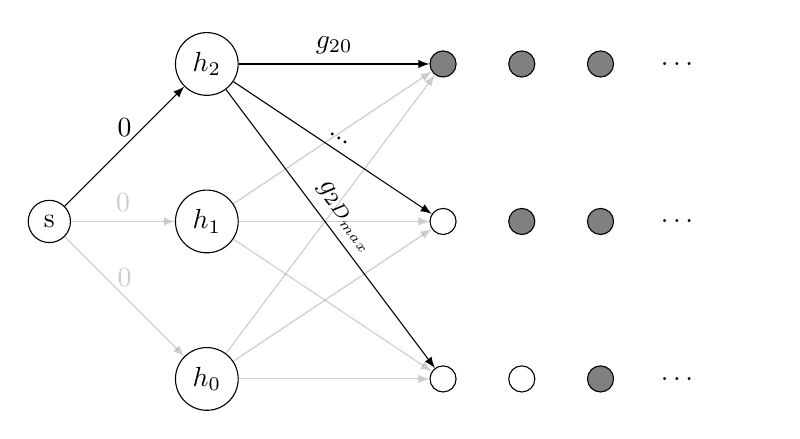
\begin{tikzpicture}[scale=1]

	\tikzstyle{vertex_closed_1} = [circle, draw=black, fill=gray] %opacity=0.3]
	\tikzstyle{vertex_closed_2} = [circle, draw=black, fill=gray]
	\tikzstyle{vertex_opened} = [circle, draw=black]

%------------------------------------------------------------
	\node[vertex_opened] (s) at (-2,2) {s};

	\node[vertex_opened] (v00) at (0,0) {$h_0$};
	\node[vertex_opened] (v01) at (0,2) {$h_1$};
	\node[vertex_opened] (v02) at (0,4) {$h_2$};
	
	\path[-latex, opacity=1]   (s) edge node[ above ] {$0$} (v02);
	\path[-latex, opacity=0.2] (s) edge node[ above ] {$0$} (v01);
	\path[-latex, opacity=0.2] (s) edge node[ above ] {$0$} (v00);
		
%------------------------------------------------------------
	
	\node[vertex_opened]   (v10) at (3,0) {};
	\node[vertex_opened]   (v11) at (3,2) {};
	\node[vertex_closed_1] (v12) at (3,4) {};
		
	\path[-latex, opacity=1] (v02) edge node[ sloped, above ] {$g_{2D_{max}}$} (v10);
	\path[-latex, opacity=1] (v02) edge node[ sloped, above ] {$...$} (v11);
	\path[-latex, opacity=1] (v02) edge node[ sloped, above ] {$g_{20}$} (v12);
	
	\path[-latex, opacity=0.2] (v01) edge node[ above ] {} (v10);
	\path[-latex, opacity=0.2] (v01) edge node[ above ] {} (v11);
	\path[-latex, opacity=0.2] (v01) edge node[ above ] {} (v12);
	
	\path[-latex, opacity=0.2] (v00) edge node[ above ] {} (v10);
	\path[-latex, opacity=0.2] (v00) edge node[ above ] {} (v11);
	\path[-latex, opacity=0.2] (v00) edge node[ above ] {} (v12);
%------------------------------------------------------------
	
	\node[vertex_opened]   (v20) at (4,0) {};
	\node[vertex_closed_1] (v21) at (4,2) {};
	\node[vertex_closed_1] (v22) at (4,4) {};
		
%------------------------------------------------------------
	
	\node[vertex_closed_1] (v30) at (5,0) {};
	\node[vertex_closed_1] (v31) at (5,2) {};
	\node[vertex_closed_1] (v32) at (5,4) {};
		
%------------------------------------------------------------

	\node[vertex_closed_1, opacity =0] (v40) at (7,0) {};
	\node[vertex_closed_1, opacity =0] (v41) at (7,2) {};
	\node[vertex_closed_1, opacity =0] (v42) at (7,4) {};
	
	\path (v30) -- node[auto=false]{\ldots} (v40);
	\path (v31) -- node[auto=false]{\ldots} (v41);
	\path (v32) -- node[auto=false]{\ldots} (v42);
	
	\end{tikzpicture}
	\captionof{figure}{граф $G$ до оптимизации}
	\label{1.4_pl_notoptimized}
\end{figure}
%1.4_pl_optimized
\begin{figure}[h!]
	\centering
	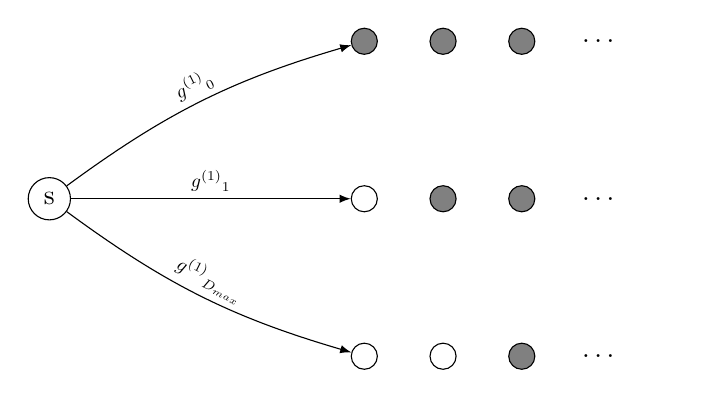
\begin{tikzpicture}[scale=1]
	\tikzstyle{vertex_closed_1} = [circle, draw=black, fill=gray]
	\tikzstyle{vertex_closed_2} = [circle, draw=black, fill=gray]
	\tikzstyle{vertex_opened} = [circle, draw=black]

%------------------------------------------------------------
	\node[vertex_opened] (s) at (-2,2) {s};
	
	\node[vertex_opened]   (v10) at (2,0) {};
	\node[vertex_opened]   (v11) at (2,2) {};
	\node[vertex_closed_1] (v12) at (2,4) {};
		
	\path[-latex, opacity=1]   (s) edge[bend right=10] node[ above, sloped, scale = 0.7 ] {${g^{(1)}}_{D_{max}}$} (v10);
	\path[-latex, opacity=1]   (s) edge node[ above, sloped, scale = 0.7 ] {${g^{(1)}}_1$} (v11);
	\path[-latex, opacity=1]   (s) edge[bend right=-10] node[ above, sloped, scale = 0.7 ] {${g^{(1)}}_0$} (v12);
%------------------------------------------------------------
	
	\node[vertex_opened]   (v20) at (3,0) {};
	\node[vertex_closed_1] (v21) at (3,2) {};
	\node[vertex_closed_1] (v22) at (3,4) {};
		
%------------------------------------------------------------
	
	\node[vertex_closed_1] (v30) at (4,0) {};
	\node[vertex_closed_1] (v31) at (4,2) {};
	\node[vertex_closed_1] (v32) at (4,4) {};
		
%------------------------------------------------------------

	\node[vertex_closed_1, opacity =0] (v40) at (6,0) {};
	\node[vertex_closed_1, opacity =0] (v41) at (6,2) {};
	\node[vertex_closed_1, opacity =0] (v42) at (6,4) {};
	
	\path (v30) -- node[auto=false]{\ldots} (v40);
	\path (v31) -- node[auto=false]{\ldots} (v41);
	\path (v32) -- node[auto=false]{\ldots} (v42);
	
	\end{tikzpicture}
	\captionof{figure}{граф $G$ после оптимизации}
	\label{1.4_pl_optimized}
\end{figure}	
\newpage

По пришествию первых $D_{max} + 2$ стерео-пар пикселей проводим аналогичные действия, но теперь уже учитываем предыдущую оптимизацию. Для каждой вершины $\sigma(3, d) \; d \in D$ находим вершину $\sigma(2, k)$, где 
$$ k = \argmin\limits_{l \in D}{\big( g^{(1)}_l +  h(2, l) + g(l, d) \big) }. $$
Отбрасываем все пути из $S$ в $\sigma(3, d), \; d \in D $, и вводим рёбра $<S, \sigma(3, d) >  \; d \in D$ c весами 
$${g^{(2)}}_d = \min\limits_{l \in D}{\big( g^{(1)}_l + h(2, l) + g(l, d) \big) },  \; \forall d \in D.$$
Этим самым снова уменьшив общее количество рёбер графа $G$ на $(D_{max})^2$.

Таким образом, при как только становятся известны первые $D_{max}+m$ стерео-пар пикселей $( m \geqslant 2)$, отбрасываем все пути из $S$ в 
$\sigma(m+1, d) \; d \in D$, заменяя их рёбрами $<S, \sigma(m+1, d) > \; \forall d \in D$, с весами 
\begin{equation}\label{1.4_f_g^i}
{g^{(m)}}_d = \min\limits_{l \in D}{\big( g^{(m-1)}_l + h(m, l) + g(l, d) \big) },  \; \forall d \in D,
\end{equation}
уменьшая количество рёбер графа $G$ ещё на $(D_{max})^2$.
\newpage

Для восстановления конечной оптимальной последовательности $\overline{d}$, нам для каждой вершины $\sigma(i, d), \; \forall \;	i = \overline{2, n}, \; d \in D$ нужно запоминать предыдущую ей ''\textit{оптимальную}'' вершину $\sigma(i-1, k)$, где 
%\begin{equation}\label{1.4_f_k}
$$k = \argmin\limits_{l \in D}{\big( {g^{(i-1)}}_l + h(i-1, l) + g(l, d) \big) }.$$
Для этого введем матрицу предыдущих оптимальных вершин $\hat{\mathcal{P}}$ размера \\
$n \times D_{max}$, где $\sigma(i-1, p_{ij}) $ -- предыдущая $\sigma(i, j)$ оптимальная вершина, \\
$\forall i \in I, j \in D$. Элементы этой матрицы находятся следующим образом:
\begin{itemize}
\item $p_{1j} = 0, \; \forall j \in D$ поскольку в вершины первого столбца можно попасть только из начальной вершины $S$, и предыдущая оптимальная вершина для них всегда одна. Конечно, можно просто исключить эти элементы из матрицы, но их наличие приводит к более красивому и простому определению остальных элементов матрицы 
$\hat{\mathcal{P}}$.
\item $p_{ij} = \argmin\limits_{l \in D}{\big( {g^{(i-1)}}_l + h(i-1, l) + g(l, j) \big) }.$
\end{itemize}
Элементы $p_{ij}$ нужно вычислять при приходе $D_{max} + i$ пары пикселей, так как при приходе следующей пары, рёбра $ g^{(i-1)}_l $ используются  
для расчёта рёбер $ g^{(i)}_l, \; \forall l \in D $ согласно формуле \ref{1.4_f_g^i} и отбрасываются.

После нахождения всех элементов $\hat{\mathcal{P}}$, можем восстановить все элементы последовательности $\overline{d}$ ---
\begin{align*}
d_n &= \argmin\limits_{l \in D}  {\big( {g^{(n-1)}}_l + h(n, l) \big) }, \\
d_{n-1} &= p_{n,d_n},\\
&\cdots\\
d_i &= p_{i,d_{n-1}}.
\end{align*}



%%-------------------------------------------------%%
\subsection{Одно из изображений известно}
%%-------------------------------------------------%%

























